% Options for packages loaded elsewhere
% Options for packages loaded elsewhere
\PassOptionsToPackage{unicode}{hyperref}
\PassOptionsToPackage{hyphens}{url}
\PassOptionsToPackage{dvipsnames,svgnames,x11names}{xcolor}
%
\documentclass[
]{article}
\usepackage{xcolor}
\usepackage{amsmath,amssymb}
\setcounter{secnumdepth}{5}
\usepackage{iftex}
\ifPDFTeX
  \usepackage[T1]{fontenc}
  \usepackage[utf8]{inputenc}
  \usepackage{textcomp} % provide euro and other symbols
\else % if luatex or xetex
  \usepackage{unicode-math} % this also loads fontspec
  \defaultfontfeatures{Scale=MatchLowercase}
  \defaultfontfeatures[\rmfamily]{Ligatures=TeX,Scale=1}
\fi
\usepackage{lmodern}
\ifPDFTeX\else
  % xetex/luatex font selection
  \setmainfont[]{Latin Modern Roman}
  \setmathfont[]{Latin Modern Math}
\fi
% Use upquote if available, for straight quotes in verbatim environments
\IfFileExists{upquote.sty}{\usepackage{upquote}}{}
\IfFileExists{microtype.sty}{% use microtype if available
  \usepackage[]{microtype}
  \UseMicrotypeSet[protrusion]{basicmath} % disable protrusion for tt fonts
}{}
\makeatletter
\@ifundefined{KOMAClassName}{% if non-KOMA class
  \IfFileExists{parskip.sty}{%
    \usepackage{parskip}
  }{% else
    \setlength{\parindent}{0pt}
    \setlength{\parskip}{6pt plus 2pt minus 1pt}}
}{% if KOMA class
  \KOMAoptions{parskip=half}}
\makeatother
% Make \paragraph and \subparagraph free-standing
\makeatletter
\ifx\paragraph\undefined\else
  \let\oldparagraph\paragraph
  \renewcommand{\paragraph}{
    \@ifstar
      \xxxParagraphStar
      \xxxParagraphNoStar
  }
  \newcommand{\xxxParagraphStar}[1]{\oldparagraph*{#1}\mbox{}}
  \newcommand{\xxxParagraphNoStar}[1]{\oldparagraph{#1}\mbox{}}
\fi
\ifx\subparagraph\undefined\else
  \let\oldsubparagraph\subparagraph
  \renewcommand{\subparagraph}{
    \@ifstar
      \xxxSubParagraphStar
      \xxxSubParagraphNoStar
  }
  \newcommand{\xxxSubParagraphStar}[1]{\oldsubparagraph*{#1}\mbox{}}
  \newcommand{\xxxSubParagraphNoStar}[1]{\oldsubparagraph{#1}\mbox{}}
\fi
\makeatother


\usepackage{longtable,booktabs,array}
\newcounter{none} % for unnumbered tables
\usepackage{calc} % for calculating minipage widths
% Correct order of tables after \paragraph or \subparagraph
\usepackage{etoolbox}
\makeatletter
\patchcmd\longtable{\par}{\if@noskipsec\mbox{}\fi\par}{}{}
\makeatother
% Allow footnotes in longtable head/foot
\IfFileExists{footnotehyper.sty}{\usepackage{footnotehyper}}{\usepackage{footnote}}
\makesavenoteenv{longtable}
\usepackage{graphicx}
\makeatletter
\newsavebox\pandoc@box
\newcommand*\pandocbounded[1]{% scales image to fit in text height/width
  \sbox\pandoc@box{#1}%
  \Gscale@div\@tempa{\textheight}{\dimexpr\ht\pandoc@box+\dp\pandoc@box\relax}%
  \Gscale@div\@tempb{\linewidth}{\wd\pandoc@box}%
  \ifdim\@tempb\p@<\@tempa\p@\let\@tempa\@tempb\fi% select the smaller of both
  \ifdim\@tempa\p@<\p@\scalebox{\@tempa}{\usebox\pandoc@box}%
  \else\usebox{\pandoc@box}%
  \fi%
}
% Set default figure placement to htbp
\def\fps@figure{htbp}
\makeatother


% definitions for citeproc citations
\NewDocumentCommand\citeproctext{}{}
\NewDocumentCommand\citeproc{mm}{%
  \begingroup\def\citeproctext{#2}\cite{#1}\endgroup}
\makeatletter
 % allow citations to break across lines
 \let\@cite@ofmt\@firstofone
 % avoid brackets around text for \cite:
 \def\@biblabel#1{}
 \def\@cite#1#2{{#1\if@tempswa , #2\fi}}
\makeatother
\newlength{\cslhangindent}
\setlength{\cslhangindent}{1.5em}
\newlength{\csllabelwidth}
\setlength{\csllabelwidth}{3em}
\newenvironment{CSLReferences}[2] % #1 hanging-indent, #2 entry-spacing
 {\begin{list}{}{%
  \setlength{\itemindent}{0pt}
  \setlength{\leftmargin}{0pt}
  \setlength{\parsep}{0pt}
  % turn on hanging indent if param 1 is 1
  \ifodd #1
   \setlength{\leftmargin}{\cslhangindent}
   \setlength{\itemindent}{-1\cslhangindent}
  \fi
  % set entry spacing
  \setlength{\itemsep}{#2\baselineskip}}}
 {\end{list}}
\usepackage{calc}
\newcommand{\CSLBlock}[1]{\hfill\break\parbox[t]{\linewidth}{\strut\ignorespaces#1\strut}}
\newcommand{\CSLLeftMargin}[1]{\parbox[t]{\csllabelwidth}{\strut#1\strut}}
\newcommand{\CSLRightInline}[1]{\parbox[t]{\linewidth - \csllabelwidth}{\strut#1\strut}}
\newcommand{\CSLIndent}[1]{\hspace{\cslhangindent}#1}



\setlength{\emergencystretch}{3em} % prevent overfull lines

\providecommand{\tightlist}{%
  \setlength{\itemsep}{0pt}\setlength{\parskip}{0pt}}



 


\usepackage{booktabs}
\usepackage{longtable}
\usepackage{array}
\usepackage{multirow}
\usepackage{wrapfig}
\usepackage{float}
\usepackage{colortbl}
\usepackage{pdflscape}
\usepackage{tabu}
\usepackage{threeparttable}
\usepackage{threeparttablex}
\usepackage[normalem]{ulem}
\usepackage{makecell}
\usepackage{xcolor}
\usepackage{arxiv}
\usepackage{orcidlink}
\usepackage{amsmath}
\usepackage[T1]{fontenc}
\makeatletter
\@ifpackageloaded{caption}{}{\usepackage{caption}}
\AtBeginDocument{%
\ifdefined\contentsname
  \renewcommand*\contentsname{Table of contents}
\else
  \newcommand\contentsname{Table of contents}
\fi
\ifdefined\listfigurename
  \renewcommand*\listfigurename{List of Figures}
\else
  \newcommand\listfigurename{List of Figures}
\fi
\ifdefined\listtablename
  \renewcommand*\listtablename{List of Tables}
\else
  \newcommand\listtablename{List of Tables}
\fi
\ifdefined\figurename
  \renewcommand*\figurename{Figure}
\else
  \newcommand\figurename{Figure}
\fi
\ifdefined\tablename
  \renewcommand*\tablename{Table}
\else
  \newcommand\tablename{Table}
\fi
}
\@ifpackageloaded{float}{}{\usepackage{float}}
\floatstyle{ruled}
\@ifundefined{c@chapter}{\newfloat{codelisting}{h}{lop}}{\newfloat{codelisting}{h}{lop}[chapter]}
\floatname{codelisting}{Listing}
\newcommand*\listoflistings{\listof{codelisting}{List of Listings}}
\makeatother
\makeatletter
\makeatother
\makeatletter
\@ifpackageloaded{caption}{}{\usepackage{caption}}
\@ifpackageloaded{subcaption}{}{\usepackage{subcaption}}
\makeatother
\usepackage{bookmark}
\IfFileExists{xurl.sty}{\usepackage{xurl}}{} % add URL line breaks if available
\urlstyle{same}
\hypersetup{
  pdftitle={Geographic Entrenchment during the 2026 Texas Primary in Harris County{,} TX},
  pdfauthor={Gabriel Brock},
  pdfkeywords={elections, spatial-networks, spatial-autocorrelation, morans-i, racial-segregation},
  colorlinks=true,
  linkcolor={blue},
  filecolor={Maroon},
  citecolor={Blue},
  urlcolor={Blue},
  pdfcreator={LaTeX via pandoc}}


\renewcommand{\today}{2026-05-01}
\newcommand{\runninghead}{A Preprint }
\title{Geographic Entrenchment during the 2026 Texas Primary in Harris
County, TX}
\def\asep{\\\\\\ } % default: all authors on same column
\author{\textbf{Gabriel
Brock}~\orcidlink{0009-0005-6958-9516}\\\\Harvard University\\Cambridge,
MA\\\href{mailto:gbrock@college.harvard.edu}{gbrock@college.harvard.edu}}
\date{2026-05-01}
\begin{document}
\maketitle
\begin{abstract}
A clear and well-documented \LaTeX~document is presented as an article
formatted for publication by ACM in a conference proceedings or journal
publication. Based on the ``acmart'' document class, this article
presents and explains many of the common variations, as well as many of
the formatting elements an author may use in the preparation of the
documentation of their work.
\end{abstract}
{\bfseries \emph Keywords}
\def\sep{\textbullet\ }
elections \sep spatial-networks \sep spatial-autocorrelation \sep morans-i \sep 
racial-segregation



\section{Introduction}\label{introduction}

It is well established that geography greatly influences politics. Place
is important at every level of politics. Even during national contests,
there is considerable variability in state-level competitiveness (McKee
and Teigen 2009). However, states cannot be considered as homogeneous
blocks that swing back and forth between Democrat and Republican or
progressively become ``Bluer'' over time. Even under demographic
changes, populations cluster together in areas far smaller than regions,
states, or counties.

Even though the state has had a state-level Republican trifecta for 20
years and has not had a Democratic Governor or U.S. Senator since 1994,
a ``blue wave'' has been forecast to over take Texas for the past 20
years. Texas leads the nation in population growth, since the state's
population has increased nearly 4 million with 95.3\% attributable to
growth of minority populations and 44\% of growth attributable to
migration from states like California. Further, many of these new
residents have settled inside of the ``Texas Triangle.'' The Triangle,
one of eleven megaregions of the United States, contains the state's
five largest cities Dallas--Fort Worth, Greater Houston, San Antonio,
and Austin. The Triangle is home to over 70\% of the state's population,
around 21 million people and much of the state's Democratic vote share
is concentrated within the region. This demographic change in addition a
changing, more diverse economy, has transformed the politics of the Lone
Star state, steadily increasing state-wide Democratic vote share even
though the party has yet to successfully win any state-wide contests.

In March 2026, Texas State Representative James Talarico of Austin
became the stat Democratic Party's nominee for United States Senate
defeating US Representative Jasmine Crockett of Dallas. The Democratic
Primary for US Senate was one of the most contentious state-wide
elections in recent history. There are several prevailing theories about
what won Talarico the election, his ability to energize young
progressives or Hispanics, but it is clear that he captured a huge
portion of the vote share in the most densely-populated region of the
state.

Talarico and Crockett both benefited from home base advantage in their
respective cities, Austin and Dallas. Talarico won Travis and Bexar
Counties by 51 and 15 points and Crockett won Dallas and Tarrant
Counties by a collective 30 points. However, this dynamic converged in
the third leg of the Triangle, Houston.

\section{Background}\label{background}

Spatial autocorrelation is the extent to which a variable is correlated
with itself through space. Tobler's First Law of Geography tells us that
``everything is related to everything else, but near things are more
related than distant things'' (Tobler 1970). As such, we expect place to
have a causal effect on voter behavior (Gimpel and Schuknecht 2004).

In metropolitan areas, observations (at the unit- and individual-level)
are often clustered together. People live near people like them.
Regardless of the variable of interest, such as racial residential
composition (e.g., \% Black), median household income (MHI), education
level, there is a general tendency for nearby observations to have
similar values, especially within urban areas. Within political
boundaries, there is significant clustering of key socioeconomic
variables (Frank 2002). Due to the inherent density of urban areas,
since VTDs in Harris County are drawn to each have ``a population
between 100 -- 5000 registered voters'' (Harris County Office of County
Administration, n.d.), the districting process creates relatively
heterogeneous rural districts and small, homogeneous urban districts
that bring together ``proximate individuals with highly correlated
preferences'' (Rodden 2010, p 332).

However, the natural contentedness of spatial networks even in dense,
urban areas is influenced by involuntary racial/ethnic/class-based
residential segregation (Anderson and Galaskiewicz 2021). Negative
spatial autocorrelation occurs when observations with dissimilar values
are dispersed (Moraga, n.d.). Positive spatial autocorrelation occurs
when observations with similar values are clustered. Urban networks are
often characterized by High-High and Low-Low autocorrelation wherein
areas with of high or low values are surrounded by areas that or similar
values (e.g., a high-income neighborhood surrounded by other high-income
neighborhoods).

Autocorrelation is especially of note because of the inherent connection
between socioeconomic context and voting behavior. The commonality
between residents of similar settings, urban, suburban or rural, produce
effects that impact voter behavior that that translate into differences
across locations Gimpel and Schuknecht (2004). There is a linkage
between the (1) clustering of social networks, (2) the demography of
these networks, and (3) how these interact to effect aspects of voter
behavior (McKee and Teigen 2009) and research has demonstrated how
demographic factors like income and race are related to key metrics of
electoral behavior like voter turnout (Saib 2017), vote change
(Bracalente and Forcina, n.d.) and partisanship Hersh and Nall (2016).
As such, it follows that these factors of voter behavior are (1) also
spatially autocorrelated and (2) able to be spatially measured in
relation to other factors.

\textbf{Sub-county Units}

Existing literature has begun to analyze voting behavior at the
sub-county level. Aggregate data analysis diminish the causal effect of
geography on electoral contexts (Wing and Walker 2010). (Gimpel and
Schuknecht 2004) emphasized the importance of voter behavior within
areas that are typically much smaller than states, which has been
supported by research analyzing smaller units (Hogrebe and Tate 2019).
(Hersh and Nall 2016) identified three issues that necessitate the study
of sub-county geographies (1) the geographic clustering of behavior, (2)
the arbitrariness of political geography, and (3) their combined
influence on redistribution preferences. As such, greater attention has
been paid to hyper-local politics, at the voter precinct- or census
tract-level. Spatial networks are incredibly sensitive to locality, even
apparently diverse neighborhoods have isolated clusters.

\textbf{Locality of Voting Behavior}

Wing and Walker (2010) building on the mechanisms established by Cho and
Rudolph (2008) argue that the same social forces that facilitate
political participation contribute to ideological reinforcement at the
local level.

Given the positive spatial autocorrelation between election results and
demographic variables, as (Hersh and Nall 2016) highlight, examining
smaller geographic units enables us to decouple socioeconomic influence
on political behavior, namely race from income. McKee and Teigan found
that location significantly relates to partisanship, affirming the claim
that regional differences persists even across urban areas Shelley and
Archer (1989) and that a mixture of compositional, contextual, and
historical effects account for the importance of place in influencing
electoral outcomes (2009). Since the turn of the century, the political
divide has been less easily explained by urban/rural differences and has
become more reliably expressed by cultural and economic factors, even in
large, dense counties (Morrill et al. 2007). Partisanship is only one
aspect of political behavior however. There is high spatial
autocorrelation of more general political participation Burnett and
Lacombe (2012) and voter turnout Saib (2017) and research provides
strong evidence of spatial clustering between general voting patterns
and demographic distributions (Rochon 2020).

Among demographic factors, race and income have an over sized impact on
voter behavior. There remains a great degree of inequality in voter
behavior correlated with income inequality. However, race conditions
this relationship especially in regard to partisanship, in predominantly
white districts, the effect of income on partisanship is greatly
minimized by race, especially in urban areas (Hersh 2015) and Blacks and
Latinos are more likely to vote in elections as their population share
increases (Fraga 2016).

\textbf{Focus on Primaries}

Primary competitiveness is highly correlated with the expected
competitiveness of the general election (Boatright and Moscardelli
2018). As such, it is important to understand \emph{why} people vote the
why they do in primary elections and what motivates any patterns in
voting behavior.

However, there remains a dearth of research focusing on intra-party
competition. Election research has demonstrated the effect of spatial
autocorrelation on election results and participation levels in the
United States. While it's important to understand the voter geography in
presidential elections, this type of micro-analysis is far more
consequential for smaller contests like municipal elections or even
Congressional elections where the electorate is densely populated. In
trying to determine the relationship between candidate vote share and
variables like race spatial analysis may produce better model fit and
more robust conclusions (Saib 2017).

In doing so, this study contributes to the existing literature in
spatial research with new assessment on the current election cycle as
well as provide insight into the spatial relationship between individual
demographic variables and partisan support at the local level.

This study seeks to understand how geography is related to voter
behavior in Harris County, TX, a place that while historically
democratic has nonetheless suffered from a high-degree of residential
segregation and in the past two decades a substantial demographic
change. Given that the 2026 Democratic primary was not influenced by
incumbency and neither front-runner to the race benefited from hometown
advantage in Harris County, we can use the county as a case study to
identify any potential spatial relationship between voter demography and
voter behavior. In doing so, this study contributes to existing spatial
research literature by furthering the assessment of the hyper-local
spatial relationship between demography and voter behavior and extending
the knowledge set regarding voter preference and intra-party
competition.

\textbf{Research Questions and Hypotheses}

The relationship between voter behavior race and other socioeconomic
variables (e.g., age, gender, income) is commonly modeled in electoral
studies. This research is guided by a set of questions interested in
more descriptive analysis of the Harris County electorate and effect of
place and demography on voting behaviors. I seek to answer the following
questions with regards to Harris County:

\begin{enumerate}
\def\labelenumi{\arabic{enumi}.}
\tightlist
\item
  How is race and income spatially clustered throughout?
\item
  To what degree, if any, is race and income spatially autocorrelated?
\item
  What is the spatial nature of key voting behaviors (turnout and voter
  preference)?
\item
  To what degree, if any, are demography and key voting behaviors
  spatially autocorrelated?
\end{enumerate}

I argue that there is a positive spatial autocorrelation between
observed voter behavior and demography in Harris County. To test this
theory, I set forth the following set of hypotheses:

\begin{itemize}
\item
  \(H_{01}\): There is no observable correlation between demography and
  candidate vote share across voter districts.
\item
  \(H_{A1}\): There is observable correlation between demography and
  candidate vote share across voter districts.
\item
  \(H_{02}\): Precinct-level residential racial composition alone is not
  a sufficient predictor of candidate vote share.
\item
  \(H_{A2}\): Precinct-level residential racial composition alone is a
  sufficient predictor of candidate vote share.
\end{itemize}

\section{Methodology}\label{methodology}

\subsection{Study Area}\label{study-area}

Harris County is composed of 1,158 voter districts organized into 8
larger regions and 1,115 census tracts (as of 2020), covering 1.77
thousand square miles. As of the 2020 Census, Harris has a population of
4.7 million, making it the most populous county in Texas and the
third-most populous county in the United States. In the 2020 general
election, Joe Biden won the county by 13\%, the widest Democratic margin
for since 1964. Though it has shifted towards Democrats in recent years,
Harris County has nevertheless voted to the right of Dallas, Travis,
Bexar, and El Paso counties, each of which has a smaller population.
However, Harris is regarded as swing county in Texas and has been
regarded as ``surprisingly liberal on topics such as immigration, gun
control and equal matrimonial rights for same-sex couples'' (Turner
2013).

\begin{figure}[H]

{\centering \pandocbounded{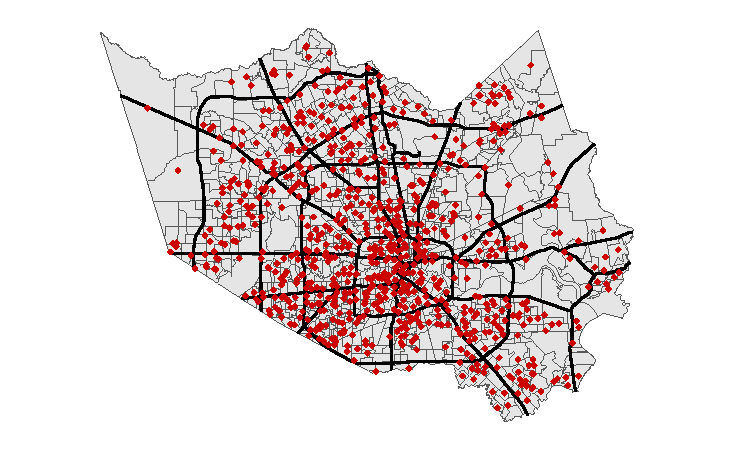
\includegraphics[keepaspectratio]{index_files/figure-pdf/Harris County Voter Districts-1.pdf}}

}

\caption{Harris County Voter Districts}

\end{figure}%

\subsection{Data Collection}\label{data-collection}

Voter precinct boundaries, voting poll locations, and major road shapes
(Figure 1) were downloaded from the Harris County OpenData portal
(\emph{Harris County Open Data}, n.d.). I used the \texttt{sf} R package
to store and convert the shapefiles for spatial analysis. I obtained
election results for the March 2026 Democratic and Republican primaries
from the Harris County Clerk's Office via the Official Canvass Report
(Harris County Clerk, n.d.). Precinct-level vote tallies were manually
entered from the report PDF to a spreadsheet, converted to a CSV file,
then loaded into R as data frames. Further tidying was conducted to
create (1) total primary activity (Democrat + Republican ballot
tallies), (2) voter turnout (total tallies / eligible voters), (3)
candidate vote share. Voter turn out and candidate vote share were both
stored as proportions to be used in further calculations.

Census Tract boundaries were obtained using the \texttt{censable} R
package based on the 2020 U.S. Census tract-boundary assessment (Kenny
2025). \texttt{censable} created a data set of population statistics for
each census tract in Harris County using 2020 decennial census data via
\texttt{censusapi} package (Recht, n.d.), importantly the data set
contains the racial cross tabs for total population and voting-aged
population (VAP).\footnote{The voting-age population (VAP) is defined by
  the Census Bureau as everyone residing in the United States, age 18
  and older. This differs from the voting-eligible population (VEP)
  coined by (McDonald 2022) to describe the population that is
  \emph{eligible} to vote excluding those who are counted in the VAP who
  are ineligible to vote; non-citizens, felons (varies), and mentally
  incapacitated persons, or unable to vote; servicepeople or civilians
  living overseas.} Additionally, each demographic variable divided
against total population to create residential proportions. This data
set was joined with more tract-level census data obtained from the
\texttt{tidycensus} package (Walker and Herman, n.d.) (e.g, median
household income, education level, \% with home internet access) via
GEOID. As highlighted by (Rochon 2020), Census tracts were used as the
unit of analysis since most meaningful demographic variables are not
recorded and/or publicly available at smaller scales of measurement like
census blocks. A full list of variables and their descriptions can be
found in the \emph{Appendix A}).

\textbf{Crosswalking}

Census geograpahy is made up of either tracts and blocks, used to
tabulate demography. Voting districts (VTD) on the other hand, are
geographies created by a non-Census entity to administer an election (U.
S. Census Bureau et al. 1994). As such, there is not a one-to-one
relationship between the boundaries of Census tracts and VTDs and it is
necessary to estimate the demographic characteristics of voter districts
According to Amos et al. (2017), there are four methods to merge spatial
data when precinct and census boundaries are non-conforming: areal
weighting, dasymetric mapping, point kriging, and kriging-based areal
interpolation. They found that dasymetric mapping was the best option
because it improved the error and fit of the general process Amos et al.
(2017, 396). This study will also use dasymetric mapping, weighting by
population density instead of land use. The process is described below:

\begin{enumerate}
\def\labelenumi{\arabic{enumi}.}
\tightlist
\item
  Trim the block group shapefile by precincts.
\item
  Calculate the area of each block, weighting by population density.
\item
  Perform a union between the shapefile to create polygons for group and
  precinct.
\item
  Calculate the area of each polygon, weighting by population density.
\item
  Divide each union shapefile are group.
\item
  Multiply this proportion by the attribute of interest for each block
  group.
\item
  Sum the quantities calculated in step 6 by precinct.
\end{enumerate}

At the time of this study, VTD identifiers were not included within
census demographic data sets provided by the US Census Bureau at the
census tract level. And while this study attempted to define census
tract boundaries by geocoded voter registration data, it was not an
accurate method for summarizing the data sets since multiple census
tracts can and do exist within a single voting precinct and this
relationship must be one to one, not one to many. Election and census
data were therefore merged based on largest areal overlap using the sf
package in R (Figure 2). It is important to note four census tracts did
not constitute a majority of any of the voter districts and were
therefore removed from the spatial layer and final analysis: tracts
221.02, 224, 229.02 and 262.02.

Finally, the non-spatial election results and census demographics were
merged to this spatial data frame shown in Figure 2 and exported as a
shapefile to be used for spatial statistical analysis. The shapefile
contained a total of forty-five discrete voting precinct boundaries,
each defined by one of twenty-eight census tracts and attributed with
the percent Democrat vote and percent demographic variable
distributions. This shapefile was used as the basis for statistical
analysis outlined in the following section.

\subsection{Project Design}\label{project-design}

\subsubsection{\texorpdfstring{Moran's \(I\)
Testing}{Moran's I Testing}}\label{morans-i-testing}

The fundamental goal of this study is the degree to which similar
demographic and electoral variables tend to occur near each other. The
most common method to assess spatial autocorrelation in areal data is
Moran's \(I\) testing Moraga (n.d.). I will Moran's \(I\) test the
variables of interest using the \texttt{spdep} R package. Specifically,
I will conduct a Local Moran's \(I\) test. Where Global Moran's \(I\)
produces one measure of the overall clustering of the spatial data, the
test assumes that spatial autocorrelation is homogeneous across the
entire study area. I want to identify any potential clusters or
anomalies in the study area. However, I calculate Local Indicators of
Spatial Association (LISA) to decompose the global measure, calculating
Local Moran's \(I\) for each spatial unit to (1) identify clustered
units (high-high or low-low) and (2) identify outlying units (high-low
or low-high), and (3) measure the influence of the unit on the magnitude
of the global statistic (Anselin 1995). The Global Moran's \(I\) is
defined as:

\[
I = \frac{N}{S_0} \cdot \frac{\sum_{i=1}^{N} \sum_{j=1}^{N} w_{ij} (x_i - \bar{x})(x_j - \bar{x})}{\sum_{i=1}^{N} (x_i - \bar{x})^2}
\]

where \(N\) is the number of spatial units (e.g., VTDs, census tracts)
indexed by \(i\) (unit) and \(j\) (neighboring units); \(x\) is the
variable of interest; \(\bar{x}\) is the mean of \(x\); \(w_{ij}\) are
the elements of a matrix of spatial weights with zeroes on the diagonal
(e.g., \(w_{ii} = 0\)); so
\(S_0 = \sum_{i=1}^{N} \sum_{j=1}^{N} w_{ij}\) or the global sum of
weights. The relationship between \(i\) and \(j\) is the between the
value of a unit and the sum of the values of \(i\)'s neighboring units,
or spatial lag. Since both VTDs and tracts are irregular polygons,
Queen-based contiguity as used to construct spatial weights, meaning
units were considered neighbors if the shared a border greater than
zero, even if it was a corner (Anselin et al. 2023).

\subsection{Descriptive Analysis}\label{descriptive-analysis}

Race and income were selected as the primary variables of interest in
this study because of the anecdotal existence is the ``Houston Arrow.''
While Houston is incredibly diverse, the 7th largest big city in the
country, it remains incredibly segregated. Historic redlining practices
and freeway development, split the city apart, separating its racial
communities and creating cleavages that still remain today. The Houston
Arrow is colloquially used to refer to the western half of the city. The
term has risen in popularity due to the arrow-like shape that forms when
mapping socioeconomic data in the city. The area contains many of the
city's wealthiest, whitest, and most connected enclaves. According to
analysis by the Kinder Institute for Urban Research tends to be have
drastically different value indexes than the immediately surrounding
area and rest of the city, that ``diversity'' is complicated on a
county-wide scale (Leah Binkovitz 2016). That

\begin{enumerate}
\def\labelenumi{\arabic{enumi}.}
\tightlist
\item
  Majority-Hispanic neighborhoods are likely to have Whites or Blacks as
  the second-most populous group in the area,
\item
  Majority-White neighborhoods are likely to have Hispanics as the
  second-most populous group. It's unlikely Blacks will be the number
  two group in a white neighborhood.
\item
  Majority-Black neighborhoods are likely to have Hispanics as the
  second-most population group. It's unlikely that Whites will be the
  number two group in a Black neighborhood.
\end{enumerate}

All this together means creates a face-value appearance that racial
networks are spatially insulated and highly clustered. Anderson and
Simburger found a moderate degree of clustering for residential minority
population share but the clustering measure of percent Black and
Hispanic were far greater than the clustering for percent Asian (the
only other substantial minority group) (2025, 6). This supports prior
conclusions that all non-White groups became increasingly segregated
from Whites and increasingly integrated with one another (Strait and
Gong 2010) and that barriers like highways are associated with greater
ethnoracial segregation and physical divisions manifest as perceived
distinctions between groups and and interethnic social connection
(Roberto and Korver-Glenn 2021).

\subsubsection{Demography}\label{demography}

\begin{figure}[H]

{\centering \pandocbounded{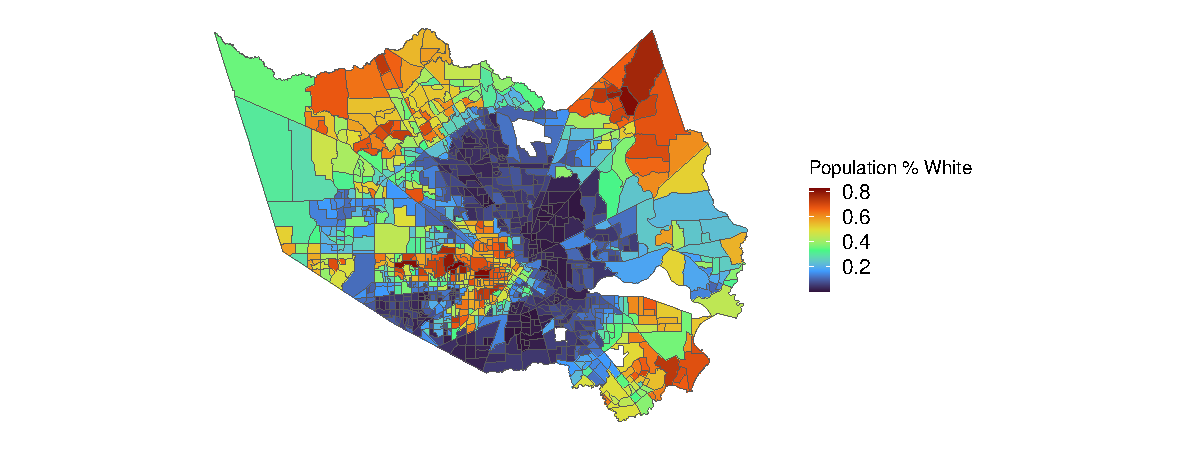
\includegraphics[keepaspectratio]{index_files/figure-pdf/unnamed-chunk-2-1.pdf}}

}

\caption{Population Share: White}

\end{figure}%

\begin{figure}[H]

{\centering \pandocbounded{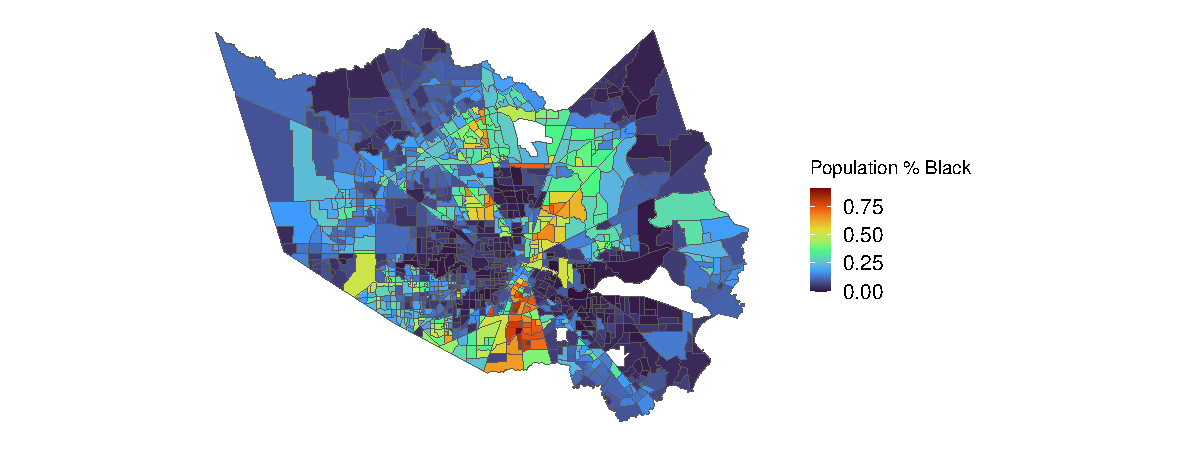
\includegraphics[keepaspectratio]{index_files/figure-pdf/unnamed-chunk-2-2.pdf}}

}

\caption{Population Share: Black}

\end{figure}%

\begin{figure}[H]

{\centering \pandocbounded{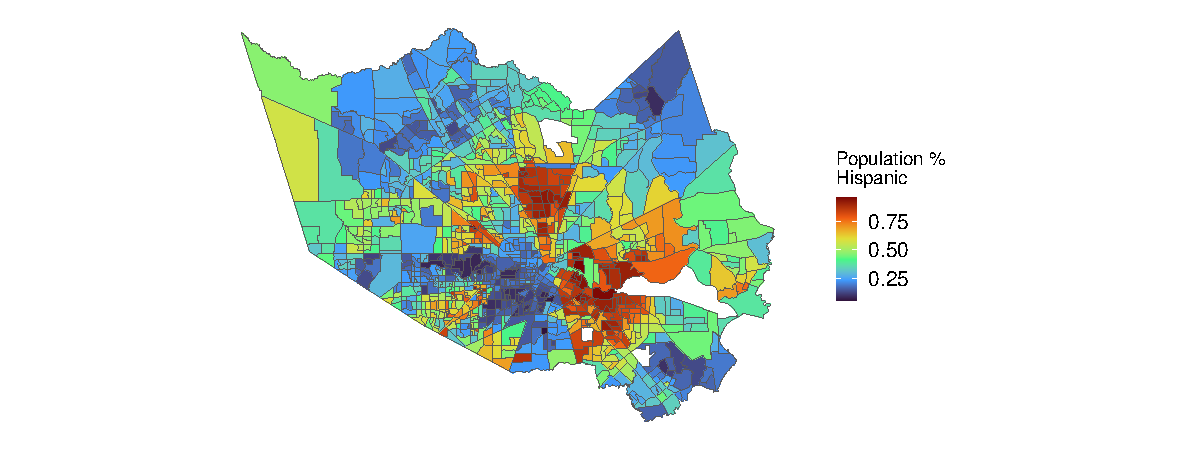
\includegraphics[keepaspectratio]{index_files/figure-pdf/unnamed-chunk-2-3.pdf}}

}

\caption{Population Share: Hispanic}

\end{figure}%

\subsubsection{Voter Turnout}\label{voter-turnout}

\begin{figure}[H]

{\centering \pandocbounded{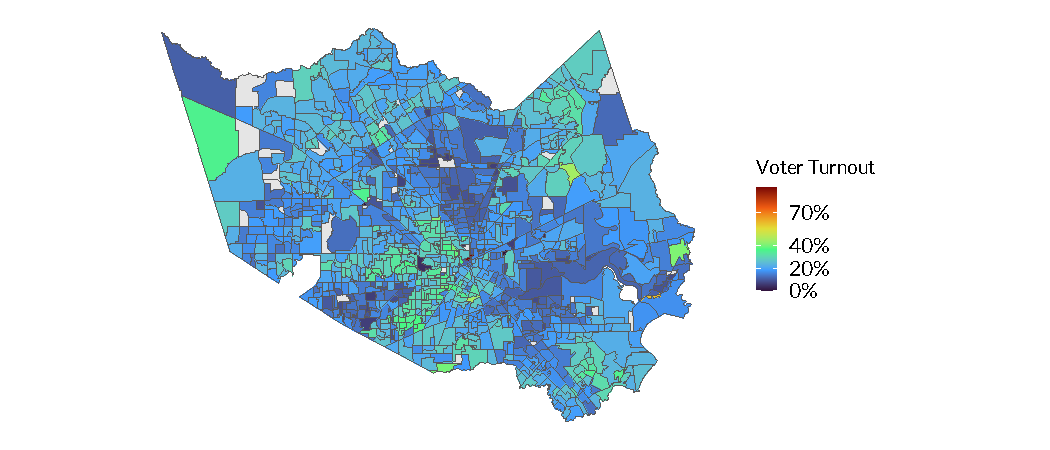
\includegraphics[keepaspectratio]{index_files/figure-pdf/Map Turnout, Precinct-Level-1.pdf}}

}

\caption{Precinct-Level Voter Turnout, 2026 Harris County Democratic
Primary}

\end{figure}%

\subsubsection{Candidate Vote Share}\label{candidate-vote-share}

\begin{figure}[H]

{\centering \pandocbounded{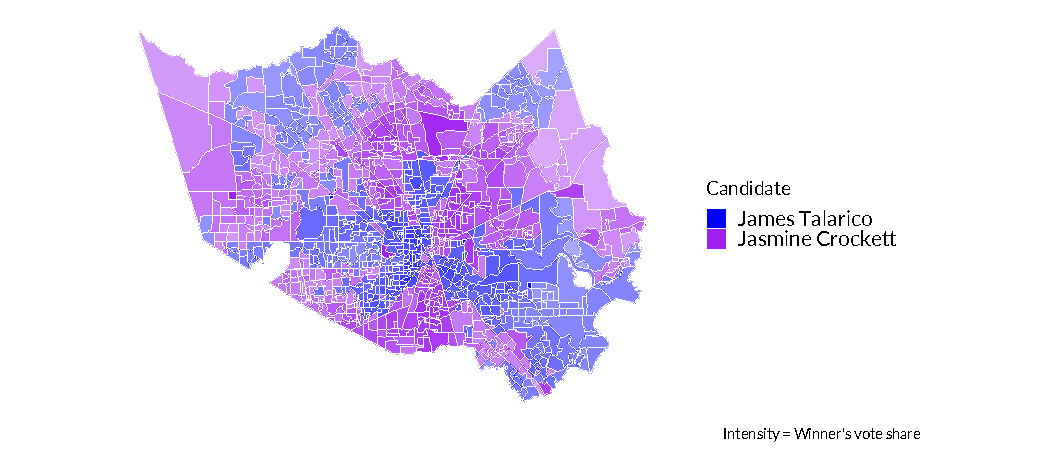
\includegraphics[keepaspectratio]{index_files/figure-pdf/Map Vote Share, Precinct-Level-1.pdf}}

}

\caption{Precinct-Level Vote Share, 2026 Harris County Democratic
Primary}

\end{figure}%

\section{Results}\label{results}

\section{Discussion}\label{discussion}

\section{Conclusion}\label{conclusion}

\newpage

\section*{References}\label{references}
\addcontentsline{toc}{section}{References}

\protect\phantomsection\label{refs}
\begin{CSLReferences}{1}{1}
\bibitem[\citeproctext]{ref-amos2017}
Amos, Brian, Michael P. McDONALD, and Russell Watkins. 2017. {``When
Boundaries Collide: Constructing a National Database of Demographic and
Voting Statistics.''} \emph{The Public Opinion Quarterly} 81: 385--400.
\url{https://www.jstor.org/stable/44507485}.

\bibitem[\citeproctext]{ref-anderson2021}
Anderson, Kathryn Freeman, and Joseph Galaskiewicz. 2021.
\emph{Racial/Ethnic Residential Segregation and Urban Spatial Networks
in the United States}. Edward Elgar Publishing.
\url{https://www.elgaronline.com/edcollchap/edcoll/9781788114707/9781788114707.00023.xml}.

\bibitem[\citeproctext]{ref-anderson2025}
Anderson, Kathryn Freeman, and Dylan Simburger. 2025. {``Racial/Ethnic
Residential Clustering, Experiences with Discrimination, and Self-Rated
Health Across the Houston Area.''} \emph{Journal of Racial and Ethnic
Health Disparities}, ahead of print, September 22.
\url{https://doi.org/10.1007/s40615-025-02651-y}.

\bibitem[\citeproctext]{ref-anselin1995}
Anselin, Luc. 1995. {``Local Indicators of Spatial
Association{\textemdash}LISA.''} \emph{Geographical Analysis} 27 (2):
93--115. \url{https://doi.org/10.1111/j.1538-4632.1995.tb00338.x}.

\bibitem[\citeproctext]{ref-anselin2023}
Anselin, Luc, Grant Morrison, Angela Li, and Karina Acosta. 2023.
\emph{Chapter 6 Contiguity-Based Spatial Weights}.
\url{https://spatialanalysis.github.io/handsonspatialdata/contiguity-based-spatial-weights.html}.

\bibitem[\citeproctext]{ref-boatright2018}
Boatright, Robert G., and Vincent G. Moscardelli. 2018. \emph{Is There a
Link Between Primary Competition and General Election Results?}
Routledge.

\bibitem[\citeproctext]{ref-bracalente}
Bracalente, Bruno, and Antonio Forcina. n.d. \emph{A Small-Area
Ecological Approach for Estimating Vote Changes and Their Determinants}.

\bibitem[\citeproctext]{ref-burnett2012}
Burnett, J. Wesley, and Donald J. Lacombe. 2012. {``Accounting for
Spatial Autocorrelation in the 2004 Presidential Popular Vote: A
Reassessment of the Evidence.''} \emph{Review of Regional Studies} 42
(1). \url{https://doi.org/10.52324/001c.8135}.

\bibitem[\citeproctext]{ref-cho2008}
Cho, Wendy K Tam, and Thomas J Rudolph. 2008. {``Emanating Political
Participation: Untangling the Spatial Structure Behind Participation.''}
\emph{British Journal of Political Science} 38 (2): 273--89.
\url{https://doi.org/10.1017/S0007123408000148}.

\bibitem[\citeproctext]{ref-fraga2016}
Fraga, Bernard L. 2016. {``Candidates or Districts? Reevaluating the
Role of Race in Voter Turnout.''} \emph{American Journal of Political
Science} 60 (1): 97--122. \url{https://doi.org/10.1111/ajps.12172}.

\bibitem[\citeproctext]{ref-frank2002}
Frank, Andrea. 2002. \emph{Using Measures of Spatial Autocorrelation to
Describe Socio-Economic and Racial Residential Patterns in US Urban
Areas}. CRC Press.

\bibitem[\citeproctext]{ref-gimpel2004}
Gimpel, James G., and Jason E. Schuknecht. 2004. \emph{Patchwork Nation:
Sectionalism and Political Change in American Politics}. The University
of Michigan Press.

\bibitem[\citeproctext]{ref-harriscountyclerk}
Harris County Clerk. n.d. \emph{Election Archives}.

\bibitem[\citeproctext]{ref-harriscountyofficeofcountyadministration}
Harris County Office of County Administration. n.d. \emph{2025
Re-Precincting}.
\url{https://oca.harriscountytx.gov/2025-Re-Precincting}.

\bibitem[\citeproctext]{ref-harrisc}
\emph{Harris County Open Data}. n.d.

\bibitem[\citeproctext]{ref-hersh2015}
Hersh, Eitan D. 2015. \emph{Hacking the Electorate: How Campaigns
Perceive Voters}. Cambridge University Press.
\url{https://doi.org/10.1017/CBO9781316212783}.

\bibitem[\citeproctext]{ref-hersh2016}
Hersh, Eitan D., and Clayton Nall. 2016. {``The Primacy of Race in the
Geography of Income-Based Voting: New Evidence from Public Voting
Records.''} \emph{American Journal of Political Science} 60 (2):
289--303. \url{https://doi.org/10.1111/ajps.12179}.

\bibitem[\citeproctext]{ref-hogrebe2019}
Hogrebe, Mark C., and William F. Tate. 2019. {``Residential Segregation
Across Metro St. Louis School Districts: Examining the Intersection of
Two Spatial Dimensions.''} \emph{AERA Open} 5 (1): 2332858419837241.
\url{https://doi.org/10.1177/2332858419837241}.

\bibitem[\citeproctext]{ref-kenny}
Kenny, Christopher T. 2025. \emph{Censable: Making Census Data More
Usable}. \url{https://christophertkenny.com/censable/}.

\bibitem[\citeproctext]{ref-leahbinkovitz2016}
Leah Binkovitz. 2016. \emph{Houston in 2016, as Told Through 5 Maps}.
Houston, TX.
\url{https://kinder.rice.edu/urbanedge/houston-2016-told-through-5-maps}.

\bibitem[\citeproctext]{ref-mcdonald2022}
McDonald, Michael P. 2022. \emph{Denominator}.
\url{https://www.electproject.org/election-data/faq/denominator}.

\bibitem[\citeproctext]{ref-mckee2009}
McKee, Seth C., and Jeremy M. Teigen. 2009. {``Probing the Reds and
Blues: Sectionalism and Voter Location in the 2000 and 2004 u. S.
Presidential Elections.''} \emph{Political Geography} 28 (8): 484--95.
\url{https://doi.org/10.1016/j.polgeo.2009.11.004}.

\bibitem[\citeproctext]{ref-moraga}
Moraga, Paula. n.d. \emph{Chapter 8 Spatial Autocorrelation \textbar{}
Spatial Statistics for Data Science: Theory and Practice with r}.
\url{https://www.paulamoraga.com/book-spatial/spatial-autocorrelation.html\#the-moran.test-function}.

\bibitem[\citeproctext]{ref-moran1950a}
Moran, P. A. P. 1950. {``Notes on Continuous Stochastic Phenomena.''}
\emph{Biometrika} 37 (1/2): 17--23.
\url{https://doi.org/10.2307/2332142}.

\bibitem[\citeproctext]{ref-morrill2007}
Morrill, Richard, Larry Knopp, and Michael Brown. 2007. {``Anomalies in
Red and Blue: Exceptionalism in American Electoral Geography.''}
\emph{Political Geography} 26 (5): 525--53.
\url{https://doi.org/10.1016/j.polgeo.2007.03.006}.

\bibitem[\citeproctext]{ref-preuss1981}
Preuss, Gary G. 1981. {``The Effects of Density and Urban Residence on
Voter Turnout.''} \emph{Population and Environment} 4 (4): 246--65.
\url{https://www.jstor.org/stable/27502946}.

\bibitem[\citeproctext]{ref-recht}
Recht, Hannah. n.d. \emph{Censusapi: Retrieve Data from the Census
APIs}.

\bibitem[\citeproctext]{ref-roberto2021}
Roberto, Elizabeth, and Elizabeth Korver-Glenn. 2021. {``The Spatial
Structure and Local Experience of Residential Segregation.''}
\emph{Spatial Demography} 9 (3): 277--307.
\url{https://doi.org/10.1007/s40980-021-00086-7}.

\bibitem[\citeproctext]{ref-rochon2020}
Rochon, Nick. 2020. {``Estimating Spatial Autocorrelation Between
Election Result and Census Demographic Distributions Within Subset of
Hennepin County, Minnesota.''} \emph{Papers in Resource Analysis} 23:
12. \url{https://gis.smumn.edu/GradProjects/RochonN.pdf}.

\bibitem[\citeproctext]{ref-rodden2010}
Rodden, Jonathan. 2010. {``The Geographic Distribution of Political
Preferences.''} \emph{Annual Review of Political Science} 13 (1):
321--40. \url{https://doi.org/10.1146/annurev.polisci.12.031607.092945}.

\bibitem[\citeproctext]{ref-saib2017}
Saib, Mahdi Salim. 2017. {``Spatial Autocorrelation in Voting
Turnout.''} \emph{Journal of Biometrics \& Biostatistics} 08 (05).
\url{https://doi.org/10.4172/2155-6180.1000376}.

\bibitem[\citeproctext]{ref-shelley1989}
Shelley, Fred M., and J. Clark Archer. 1989. {``Sectionalism and
Presidential Politics: Voting Patterns in Illinois, Indiana, and
Ohio.''} \emph{Journal of Interdisciplinary History} 20 (2): 227.
\url{https://doi.org/10.2307/204833}.

\bibitem[\citeproctext]{ref-strait2010}
Strait, John B., and Gang Gong. 2010. {``Ethnic Diversity in Houston,
Texas: The Evolution of Residential Segregation in the Bayou City,
1990{\textendash}2000.''} \emph{Population Review} 49 (1).
\url{https://muse.jhu.edu/pub/42/article/387344}.

\bibitem[\citeproctext]{ref-tobler1970}
Tobler, W. R. 1970. {``A Computer Movie Simulating Urban Growth in the
Detroit Region.''} \emph{Economic Geography} 46: 234--40.
\url{https://doi.org/10.2307/143141}.

\bibitem[\citeproctext]{ref-turner2013}
Turner, By Allan. 2013. \emph{Survey Finds Area Growing in 'Tolerant
Traditionalists'}.
\url{https://www.houstonchronicle.com/news/houston-texas/houston/article/Survey-finds-area-growing-in-tolerant-4456041.php}.

\bibitem[\citeproctext]{ref-turner1908}
Turner, Frederick J. 1908. {``Is Sectionalism in America Dying Away?''}
\emph{American Journal of Sociology} 13 (5): 661--75.
\url{https://www.jstor.org/stable/2762578}.

\bibitem[\citeproctext]{ref-u.s.censusbureau1994}
U. S. Census Bureau, Economics, and Statistics Administration. 1994.
\emph{Voting Districts}.
\url{https://www2.census.gov/geo/pdfs/reference/GARM/Ch14GARM.pdf}.

\bibitem[\citeproctext]{ref-walker}
Walker, Kyle E., and Matt Herman. n.d. \emph{Tidycensus: Load US Census
Boundary and Attribute Data as 'Tidyverse' and 'Sf'-Ready Data Frames}.

\bibitem[\citeproctext]{ref-wing2010}
Wing, Ian Sue, and Joan L. Walker. 2010. \emph{The Geographic Dimensions
of Electoral Polarization in the 2004 u.s. Presidential Vote}. Edited by
Antonio Páez, Julie Gallo, Ron N. Buliung, and Sandy Dall'erba. Advances
in Spatial Science. Springer Berlin Heidelberg.
\url{http://link.springer.com/10.1007/978-3-642-03326-1}.

\bibitem[\citeproctext]{ref-yandri2017}
Yandri, Pitri. 2017. {``The Political Geography of Voters and Political
Participation: Evidence from Local Election in Suburban Indonesia.''}
\emph{Indonesian Journal of Geography} 49 (1): 57.
\url{https://doi.org/10.22146/ijg.11315}.

\end{CSLReferences}




\end{document}
